\documentclass[12pt]{article}
\usepackage[a4paper, total={7.5in, 11in}]{geometry}
\usepackage{array}
\usepackage{graphicx, subfig, wrapfig, fancyhdr, lastpage, multicol ,color,arydshln,makecell}

\newcommand\headerMe[2]{\noindent{}#1\hfill#2}
\usepackage[mathscr]{euscript}
\usepackage{tabularray}

\setlength{\columnseprule}{1pt}
\def\columnseprulecolor{\color{blue}}


\pagestyle{fancy}
\fancyhf{}

\cfoot{ \vspace{-0.8cm}\em{Page \thepage \hspace{1pt} / \pageref{LastPage}}}
\begin{document}

\headerMe{Royaume du Maroc}{année scolaire \emph{2022-2023}}\\
\headerMe{Ministère de l'Éducation nationale, }{  Professeur :\emph{Zakaria Haouzan}}\\
\headerMe{du Préscolaire et des Sports}{Établissement : \emph{Lycée SKHOR qualifiant}}\\
%\vspace{-1cm}
\begin{center}
Devoir Surveillé  N°2 - S2 \\
    2ème année baccalauréat Sciences physiques\\
Durée 2h00
\\
    \vspace{.2cm}
\hrulefill
\Large{Chimie 7pts - 45min}
\hrulefill\\

    %\emph{Les deux parties sont indépendantes}
\end{center}
%end Headerss------------------------
%__________________Chimie ______________________-
%%%%%%%+_+_+_+_+_+_+_+_+_Partie1

 \section*{Partie 1 : Gaz d’une grande pureté. \dotfill(07pts)- 45min }
\begin{wrapfigure}[5]{r}{0.32\textwidth}
  \begin{center}
	  \vspace{-0.6cm}
	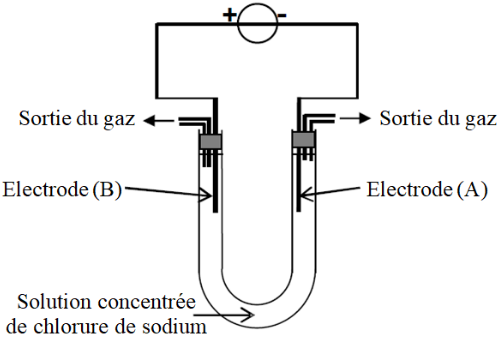
\includegraphics[width=0.32\textwidth]{./img/ex00.png}
  \end{center}
\end{wrapfigure}
	   \emph{L'électrolyse permet d'obtenir des gaz d'une grande pureté.
On réalise l'électrolyse d'une solution concentrée de chlorure de sodium
$Na^+_{(aq)} + Cl^-_{(aq)}$, on obtient un dégagement de dichlore au voisinage de l’une des
électrodes, et dégagement de dihydrogène au voisinage de l'autre électrode, de plus
que le milieu réactionnel \\devient basique au cours de la transformation chimique.}

\begin{itemize}
	\item Les couples intervenants dans la transformation\\ chimique : $(H_2O_{(l)})/H_{(g)})$ et $(Cl_{2(g)}/Cl^-_{(aq)})$
	\item Le faraday $\mathscr{F}=9,65.10^4 C.mol^{-1}$
	\item Le volume molaire dans les conditions de l’expérience :$V_m = 25,0L.mol^{-1}$
\end{itemize}
La figure ci-contre représente le
dispositif expérimental utilisé pour
réaliser cette électrolyse.


\begin{tabular}{c | c}
		1 & \makecell[l]{\textbf{1. }Déterminer laquelle parmi les
électrodes (A) et (B) celle qui
joue le rôle de l'anode et celle\\
qui joue le rôle de la cathode.}\\

			1 & \makecell[l]{\textbf{2. }Ecrire l’équation de la réaction
ayant lieu au voisinage de
chaque électrode, et l'équation\\
bilan de cette électrolyse.}\\

 1 & \makecell[l]{\textbf{3. } Le générateur alimente le circuit avec un courant électrique d'intensité constante
	$I = 3A$.\\Calculer la quantité d’électricité Q débitée au cours de $\Delta{t} = 80 min$. 
}\\

2 & \makecell[l]{\textbf{4. } Calculer le volume du dichlore $Cl_2$ formé pendant la durée $\Delta{t} = 80 min$.}\\
	
2 & \makecell[l]{\textbf{5. } Calculer le volume du dihydrogène $H_2$ formé pendant la durée $\Delta{t} = 80 min$.}\\
\end{tabular}
%\begin{center}
%\begin{tabular}{ |c| c|}
%\hline
%\textbf{Couple acide/base} &\textbf{ Valeur de $pK_A$}\\\hline
	%$HCOOH / HCOO^-$  & 3,75 \\\hline
	%$C_6H_5COOH/C_6H_5COO^-$ &4,2\\\hline
	%$CH_3COOH/CH_3COO^-$&  4,75 \\\hline
	%$CH_3-CH_2-COOH/CH_3-CH_2-COO^-$ &4,9 \\\hline

%\end{tabular}
%\end{center}

%\begin{tabular}{c|l}
	%0,5 & \makecell[l]{\textbf{3. }Déterminer le volume
	%$V_{b1}$ de la solution $S_b$ versée, au cours du dosage, pour que: $\frac{[AH]}{[A^-]} = 2,24$ . }\\
%\end{tabular}

%\hrulefill
%\Large{Physique 13pts/78min}
%\hrulefill\\
%\newpage
\begin{center}
    %\vspace{.60cm}
\hrulefill
\Large{Physique 13pts - 75min}
\hrulefill\\
    %\emph{Les  parties sont indépendantes}
\end{center}

%\vspace{-1cm}
\section*{Exercice 1–Chute d’un solide dans le champ de pesanteur\dotfill(5pts)}

%\begin{wrapfigure}[9]{r}{0.25\textwidth}
  %\begin{center}
	  %\vspace{-1cm}
	%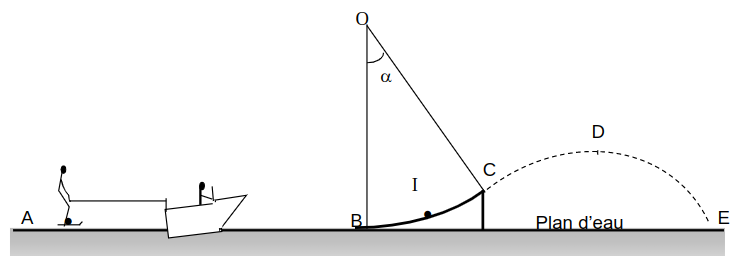
\includegraphics[width=0.19\textwidth]{./img/img01.png}
	%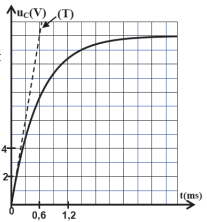
\includegraphics[width=0.25\textwidth]{./img/img02.png}
  %\end{center}
%\end{wrapfigure}

	\begin{wrapfigure}[7]{r}{0.32\textwidth}
  \begin{center}

	  \vspace{-1.6cm}
	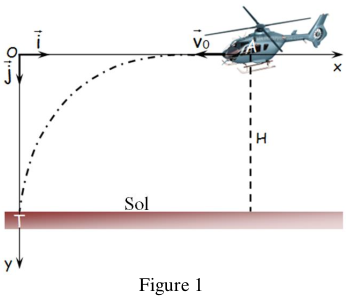
\includegraphics[width=0.32\textwidth]{./img/ex_02.png}
  \end{center}
\end{wrapfigure}
	\emph{Les hélicoptères sont parfois utilisés pour approvisionner, d’aides humanitaires, les
zones sinistrées non joignables par voies terrestres.}

Un hélicoptère vole à une altitude H
constante par rapport au sol, avec une
vitesse horizontale $\vec{V_0}$ constante. Il
fait tomber un paquet d’aliments de
centre de gravité $G_0$, qui tombe sur le
sol au point T. (Figure 1)
On étudie le mouvement de G0 dans
un
repère
orthonormé $(R,O,\vec{i}, \vec{j})$
supposé galiléen.

\textbf{On donne :} $g = 10 m.s^{-2}$  ;  $H=405m$ ; On néglige les dimensions du paquet.

\textbf{\underline{Partie 1 : Etude de la chute libre : }}
On néglige les forces liées \\à l’action de l’air sur le paquet.
Le paquet tombe, à l’instant $t = 0$, à \\partir du point $A(x_A = 450 m, y_A = 0)$, avec une
vitesse initiale horizontale $\vec{V_0}$ de valeur $V_0 = 50 m.s^{-1}$.

\begin{tabular}{c|l}	
	1 & \makecell[l]{\textbf{1.1. } Par application de la deuxième loi de Newton, trouver les équations
		horaires x(t) et y(t) du \\mouvement de $G_0$ dans le repère $(R,O,\vec{i}, \vec{j})$.
 }\\

	0,75 & \makecell[l]{\textbf{1.2. } Déterminer l’instant d’arrivée du paquet au sol.
 }\\
	
	0,5 & \makecell[l]{\textbf{1.3. } Trouver l’équation de la trajectoire du mouvement de $G_0$.
}\\
\end{tabular}


\textbf{\underline{Partie 2 :Etude de la chute avec frottements }}

Pour ne pas se détériorer lors du choc avec le sol, un paquet d’aliments a été attachée
à un parachute lui permettant une descente lente. L’hélicoptère reste immobile à une
altitude H au-dessus du point O. Le paquet et son parachute tombent verticalement
sans vitesse initiale à l’instant $t_0 = 0$.
L’air exerce des forces de frottements modélisées par la relation : $\vec{f}$=$-100.\vec{v}$ , où $\vec{v}$
représente le vecteur vitesse du paquet à l’instant t.
On néglige la poussée d’Archimède pendant la chute.

\textbf{On donne : } La masse du système {caisse + parachute} : $m = 150 kg$.
  
\begin{center}
	  \vspace{-0.2cm}
	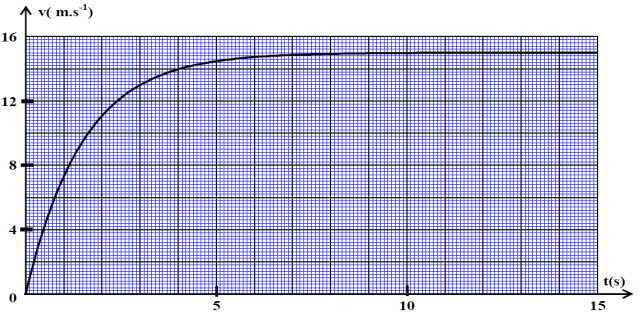
\includegraphics[width=0.61\textwidth]{./img/ex_00_2.png}
  \end{center}

  \vspace{-0.4cm}
\begin{tabular}{c|l}	
	1,25 & \makecell[l]{\textbf{2.1. } Etablir l’équation différentielle vérifiée par la vitesse du centre d’inertie $G_1$ du
		système \\dans le repère $(R,O,\vec{i}, \vec{j})$ .
 }\\

	0,25 & \makecell[l]{\textbf{2.2. } La courbe de la figure 2, représente les variations de la vitesse du centre
d’inertie $G_1$ du \\système en fonction du temps. Déterminer la valeur de la vitesse
limite $V_{lim}$ et celle du temps \\caractéristique $\tau$ de chute.
 }\\
	
	0,25 & \makecell[l]{\textbf{2.3. } Estimer la durée du régime initial.}\\
	1 & \makecell[l]{\textbf{2.4. } Par utilisation de la méthode d’Euler et le tableau suivant, déterminer les valeurs
\\de la vitesse $v_4$ et de l’accélération $a_4$.
}\\
\end{tabular}





\begin{center}
\begin{tabular}{ |c|c|c|c|c|c|c|c| } 
 \hline
 $t_i(s)$		 & 0&0,1 &0,2& 0,3& 0,4& 0,5& 0,6\\\hline
 $V_i(m/s)$      &0 & 1,0 & 1,93 & 2,80 &$v_4$&4,37&5,08\\\hline 
 $a_i(m.s^{-2})$ & 10,0& 9,33 & 8,71 &8,12&$a_4$&7,07& 6,60\\\hline  
 \hline
\end{tabular}
\end{center}



\section*{Exercice 2–Mouvement d’une particule chargée \dotfill(2,5pts)}


	\begin{wrapfigure}[4]{r}{0.2\textwidth}
  \begin{center}
	  \vspace{-0.8cm}
	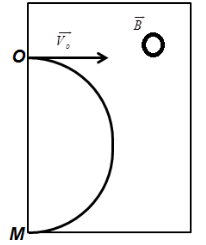
\includegraphics[width=0.2\textwidth]{./img/ex_00.png}
  \end{center}
\end{wrapfigure}

Les ions $O^{2-}$ pénètrent dans une région de l'espace où règne un champ $\vec{B}$(perpendiculaire au plan de la figure). Avec une vitesse
magnétique uniforme  $V_0 =1,6.10^4.m.s^{-1}$

\textbf{Données :} L'intensité du champs magnétique $B= 0,1T$ ; La charge élémentaire $e = 1, 6.10^{-19} C$



\begin{tabular}{c|l}	

1	  & \makecell[l]{\textbf{1. }Donner les caractéristiques de la force magnétique $\vec{F_m}$.
}\\
	0,25 & \makecell[l]{\textbf{2. }Déterminer le sens du champs magnétique $\vec{B}$.
 }\\
	0,75 & \makecell[l]{\textbf{3. }En appliquant la deuxième loi de newton dans un référentiel galiléen,
		\\montrer que le mouvement des ions $O^{2-}$ est circulaire uniforme.}\\
	 0,5& \makecell[l]{\textbf{4. }Calcule la masse d'ion $O^{2-}$ (On donne $OM = 4 cm$ )
}\\
\end{tabular}

\newpage
\section*{Exercice 3 – Mouvement des satellites et planètes \dotfill(5,5pts)}

	\begin{wrapfigure}[4]{r}{0.26\textwidth}
  \begin{center}
	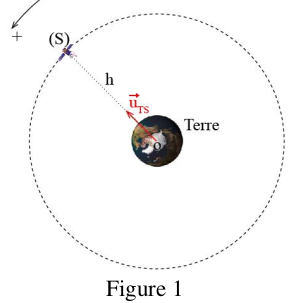
\includegraphics[width=0.26\textwidth]{./img/ex__00 .png}
  \end{center}
\end{wrapfigure}

\emph{ Le pigeon bleu est un satellite artificiel marocain assurant le contrôle des frontières
géographiques du royaume et les télécommunications. Il a été instauré par des
experts du centre royal de télédétection spatiale en collaboration avec experts
internationaux.}

\emph{Le pigeon bleu a été mis en orbite le 10 décembre 2001 à une altitude h du sol. \\Ce
satellite artificiel (S) effectue environ 14 tours autours de la terre par jour. }

\textbf{Données} : 

\begin{itemize}
	\item On assimile l’orbite de (S) à un cercle de centre O, et on étudie son mouvement
dans le repère géocentrique.
\item La Terre est considérée comme une sphère à répartition sphérique de masse.
\item  On néglige les dimensions de (S) devant sa distance au centre de la Terre.

\item La valeur de la constante de gravitation universelle : $G = 6,67.10^{-11}$ (SI) ;
\item  La valeur du rayon de la Terre : $r_T = 6350 km$ ;
\item  La valeur de l’intensité de pesanteur à la surface
	de la Terre : $g_0 = 9,8 m.s^{-2}$ ;
\item La valeur de la période de rotation de la Terre
autour de son axe polaire : $T = 86164 s$ et La valeur de l’altitude : $h = 1000 km$ ;
\item $\vec{u_TS}$ : Vecteur unitaire dirigé de O vers S.

\end{itemize}

\begin{tabular}{c|l}	

	0,5  & \makecell[l]{\textbf{1. }Recopier le schéma de la figure 1, et représenter dessus le vecteur vitesse $\vec{V_S}$ du
satellite\\ artificiel, et le vecteur force d’attraction universelle modélisant l’action
de la Terre sur (S).}\\
	0,25  & \makecell[l]{\textbf{2. }Donner l’expression vectorielle de la force d’attraction universelle modélisant
l’action \\de la Terre sur (S).}\\

	 0,5 & \makecell[l]{\textbf{3. }Ecrire dans le repère de Freinet, l’expression du vecteur accélération du
mouvement de (S).
}\\

	   & \makecell[l]{\textbf{4. } Par application de la 2ème loi de Newton sur le mouvement du centre de gravité
\\du satellite (S) :}\\
	  0,75 & \makecell[l]{\textbf{4.1 }Montrer que le mouvement de (S) est circulaire uniforme.
 }\\
	  0,75 & \makecell[l]{\textbf{4.2 }Ecrire l’expression de $V_S$ en fonction de $g_0$, $r_T$, et $h$. Calculer sa valeur.
 }\\
	  0,5 & \makecell[l]{\textbf{5. }Montrer que la masse de la terre est : $M_T = 6.10^{24} kg$.
}\\
	  0,75 & \makecell[l]{\textbf{6. }Montrer que le satellite artificiel n’apparait pas immobile par rapport à un
Un autre \\satellite artificiel (S’) tourne autour de la Terre avec une vitesse
angulaire $\omega$, et apparait\\ immobile par rapport à un observateur terrestre.
Le satellite (S’) envoie à la terre des \\photos utilisées dans les prévisions météo.
}\\
	  0,75 & \makecell[l]{\textbf{7. } Montrer que : $\omega^2.(r_T + z)^3 = Cte$ où est la distance séparant le sol terrestre du
satellite (S’).
}\\
	  0,75 & \makecell[l]{\textbf{8. }Trouver la valeur de z.}\\

\end{tabular}




\end{document}
